\documentclass{report}
    \title{50004 - Operating Systems - Lecture 1}
    \author{Oliver Killane}
    \date{12/10/21}

%===========================COMMON FORMAT & COMMANDS===========================
% This file contains commands and format to be used by every module, and is 
% included in all files.
%===============================================================================

%====================================IMPORTS====================================
\usepackage[a4paper, total={6in, 8in}]{geometry}
\usepackage{graphicx, amssymb, amsfonts, amsmath, xcolor, listings, tcolorbox, multirow, hyperref}
%===============================================================================

%====================================IMAGES=====================================
\graphicspath{{image/}}

% \centerimage{options}{image}
\newcommand{\centerimage}[2]{\begin{center}
    \includegraphics[#1]{#2}
\end{center}}
%===============================================================================

%=================================CODE LISTINGS=================================
\definecolor{codebackdrop}{gray}{0.9}
\definecolor{commentgreen}{rgb}{0,0.6,0}
\lstset{
    inputpath=code, 
    commentstyle=\color{commentgreen},
    keywordstyle=\color{blue}, 
    backgroundcolor=\color{codebackdrop}, 
    basicstyle=\footnotesize,
    frame=single,
    numbers=left,
    stepnumber=1,
    showstringspaces=false,
    breaklines=true,
    postbreak=\mbox{\textcolor{red}{$\hookrightarrow$}\space}
}

% Create a code listing for a single line
% \codeline{language}{line}{file}
\newcommand{\codeline}[3]{\lstinputlisting[language=#1, firstline = #2, lastline = #2]{#3}}

% Create a code listing for a given language & file
% \codelist{language}{file}
\newcommand{\codelist}[2]{\lstinputlisting[language=#1]{#2}}
%===============================================================================

%================================TEXT STRUCTURES================================
% Marka a word as bold
% \keyword{important word}
\newcommand{\keyword}[1]{\textbf{#1}}

% Creates a section in italics
% \question{question in italics}
\newcommand{\question}[1]{\textit{#1} \\ }

% Creates a box with title for side notes.
% \sidenote{title}{contents}
\newcommand{\sidenote}[2]{\begin{tcolorbox}[title=#1]#2\end{tcolorbox}}

% Creates an item in an itemize or enumerate, with a paragraph after
% \begin{itemize}
%     \bullpara{title}{contents}
% \end{itemize}
\newcommand{\bullpara}[2]{\item \textbf{#1} \ #2}

% Creates a compact list (very small gaps between items)
% \compitem{
%     \item item 1
%     \item item 2
%     \item ...
% }
\newcommand{\compitem}[1]{\begin{itemize}\setlength\itemsep{-0.5em}#1\end{itemize}}

% Creates a link to the lecture for use at the start of the notes document
\newcommand{\lectlink}[1]{\sidenote{Lecture Recording}{
    Lecture recording is available \href{#1}{here}
}}
%===============================================================================


%==============================SYNTAX HIGHLIGHTING==============================
\newcommand{\fun}[1]{\textcolor{blue}{\textbf{#1}}}
\newcommand{\file}[1]{\textcolor{green}{\textbf{#1}}}
\newcommand{\struct}[1]{\textcolor{orange}{\textbf{#1}}}
\newcommand{\var}[1]{\textcolor{purple}{\textbf{#1}}}
\newcommand{\const}[1]{\textcolor{red}{\textbf{#1}}}
%===============================================================================

%==============================THREAD HIGHLIGHTING==============================
\newcommand{\threada}[1]{\textcolor{green}{\textbf{#1}}}
\newcommand{\threadb}[1]{\textcolor{red}{\textbf{#1}}}
%===============================================================================

%============================DISPLAYING THREAD CODE=============================
\newcommand{\threadlist}[3]{
    \codelist{#1}{#2 init.#3}
    \begin{minipage}[t]{0.45\textwidth}
        \codelist{#1}{#2 A.#3}
    \end{minipage}
    \hfill
    \begin{minipage}[t]{0.45\textwidth}
        \codelist{#1}{#2 B.#3}
    \end{minipage}
}
%===============================================================================

\begin{document}
    \maketitle
    \sidenote{Lecture Recording}{
        Lecture recording is available \href{https://imperial.cloud.panopto.eu/Panopto/Pages/Viewer.aspx?id=90571bc3-0ec6-4452-9461-adbf00c863f3}{here}
    }
    \section*{Introduction}
        Covering the theoretical side of OS, with many concepts to be implemented in the Pintos lab.
        \subsection*{Course Delivery}
            \begin{center}
                \begin{tabular}{r l}
                    Week & Form \\
                    \hline
                    2-3 & Remote live lectures on teams (Tues and Thurs) \\
                    4 & No lectures \\
                    5-11 & Hybrid lectures (Teams \& Huxley) \\
                \end{tabular}
            \end{center}
            \subsubsection*{Part 1 - Dr Pietzuch}
                \begin{itemize}
                    \item Overview and Introduction
                    \item Processes and Threads
                    \item Overview and Introduction
                \end{itemize}
                \subsubsection*{Part 2 - Luis}
                \begin{itemize}
                    \item Memory Management
                    \item Device Management
                    \item Disk Management
                    \item File Systems
                    \item Security
                    \item Virtualisation
                \end{itemize}
            \subsubsection*{Recommended Reading}
                \begin{enumerate}
                    \item Modern Operating Systems
                    \item Operating Systems: 3 easy pieces (free online)
                    \item Understanding the Linux Kernel
                    \item Inside Windows NT \& 2000
                \end{enumerate}
    
    \section*{Computer Architecture Overview}
        OS provides a clean interface for different types of applications to run of different hardware.
        \\ \centerline{\textit{OS provides resource management and useful abstractions.}}
        \begin{center}
            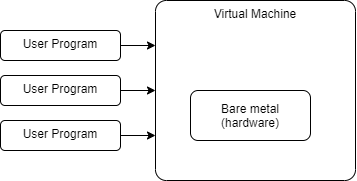
\includegraphics[scale = 0.6]{OS VM.png} \\
        \end{center}
        \begin{center}
            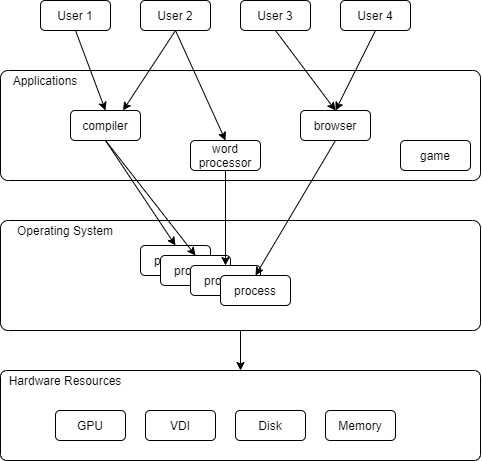
\includegraphics[scale = 0.6]{OS diagram.png}
        \end{center}
    \section*{OS Characteristics}
        The OS must be able to:
        \begin{itemize}
            \item Must share Data, programs and hardware (time and space multiplexing)
            \item Must offer resource allocation (efficient and fair use of memory, CPU etc)
            \item Must offer simultaneous access to resources, or if this is not possible, enforce mutual exclusion.
            \item Must protect against accidental or malicious corruption of Data.
        \end{itemize}
        Can also support concurrency (logical or actual)
        \begin{itemize}
            \item Support simultaneous activities occurring, e.g multiple users \& programs 
            \item Can switch activities at any arbitrary time, and must ensure this does not result in program failures
            \item Ensure safe concurrency through primitives (e.g semaphores, locks)
        \end{itemize}
        The OS must also take into account non-determinism, as it cannot predict what interrupts/events will occur and when. (events occur in an unpredictable order)
        \\
        \\ Also needs to consider persistent storage (e.g HDD, SSD etc).
        \begin{itemize}
            \item easy access to files through user-defined names.
            \item Enforces access controls (permissions to read, write, copy, etc).
            \item Can Protect against failure (e.g backups).
            \item Manage storage devices, partitions etc.
        \end{itemize}
    \section*{OS Structure}
        \subsubsection*{Monolithic}
            Whole OS is on executable. File system, drivers etc are built into the kernel and run with privilege.
        \subsubsection*{Microkernel}
            \begin{itemize}
                \item Kernel provides some abstraction, manages resources, but many services run as servers (e.g file system, drivers, etc).
                \item IPC slow, so lower performance than monolithic.
                \item More reliable.
            \end{itemize}
        \subsubsection*{Hybrid Kernel}
            Mix of the two above, used by OS's such as windows.
    \section*{Linux}
        Linux is a variant of Unix, developed as a monolithic version of the Minix kernel.
        \begin{itemize}    
            \item System calls implemented by putting args in registers \& on the stack and issuing a trap.
            \item Supports many programs through GNU (GNU's not unix) project.
            \item Interrupt handlers are the primary method of interacting with devices.
            \item Supports dynamically loadable modules.
            \item exposes many devices and services as files.
        \end{itemize}
    \section*{Windows}
        A hybrid kernel, NT replaced MS-DOS and was inspired by VMS.
        \begin{center}
            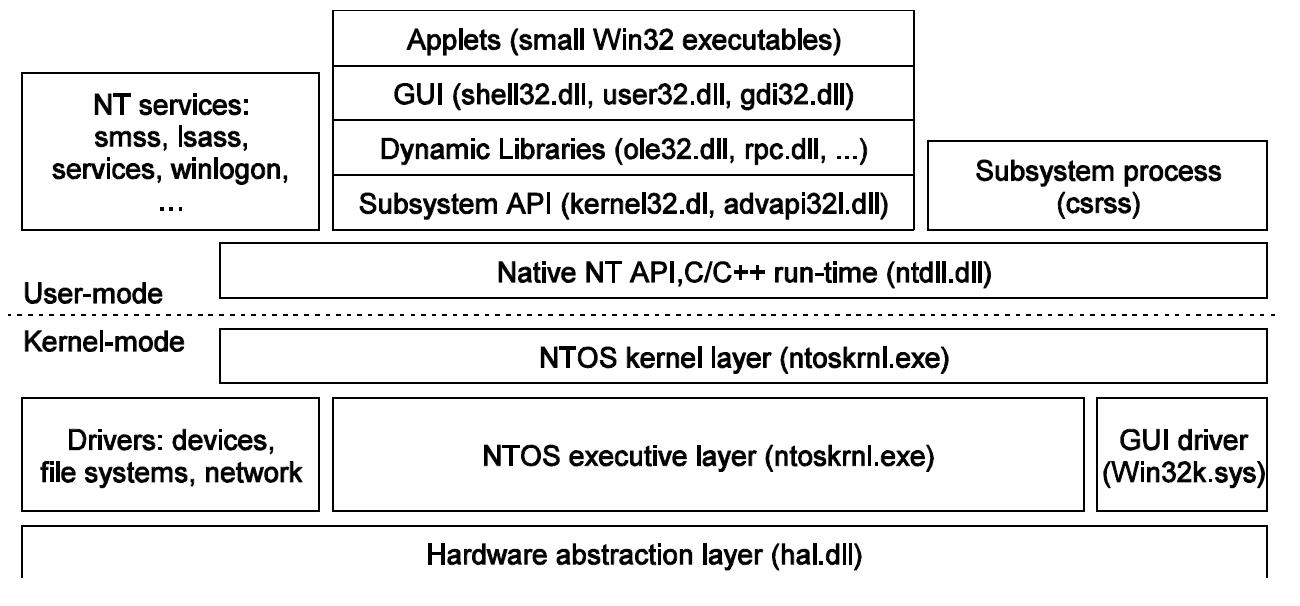
\includegraphics[width=\textwidth]{windows kernel.png}
        \end{center}
        \keyword{NTOS} is loaded from ntoskrnl.exe (windows NT operating system kernel executable) at boot.
        \\ It consists of two layers:
        \begin{enumerate}
            \item Executive - Most of the services.
            \item Kernel Thread scheduling \& synchronisation, traps, interrupt handlers, and CPU management.
        \end{enumerate}
        There is also a \keyword{HAL} (Hardware Abstraction Layer) that abstracts away DMA (direct memory access) operations, BIOS config \& CPU types. This in theory makes windows easy to poert to new devices and architectures. However in practice for mainly commercial reasons this has not occurred.
\end{document}
